

\subsection{Design}
\label{shreds:sec:design}
%We design and implement a system that enables shreds for Linux/ARM platforms. Our system consists of a compilation toolchain (S-compiler) and a dynamic loadable kernel extension (S-driver). Developers can adopt shreds in their programs using a set of simple APIs: two APIs for entering and exiting a shred; two APIs for allocating and freeing memory in an s-pool. S-compiler is needed to build programs that contain shreds. S-compiler performs the code analysis and instrumentation. During runtime, S-driver handles shred creations and terminations. It manages and protects s-pools. Our design makes a novel use of memory domains, an under-exploited feature in ARM CPUs, to efficiently protect s-pools and shred executions.
\subsubsection{Shred APIs and Usages}
Application developers use shreds and s-pools via the following intuitive APIs: 

\vspace{.1in}
\indent\indent {\tt err\_t }{\btt shred\_enter}{\tt (int {\itt pool\_desc})};   \\
\indent\indent {\tt err\_t }{\btt shred\_exit}{\tt ()};     \\
\indent\indent {\tt void * }{\btt spool\_alloc}{\tt (size\_t {\itt size})};   \\
\indent\indent {\tt void  }{\btt spool\_free}{\tt (void *{\itt ptr})};     
\vspace{.1in}

These APIs internally make requests to S-driver via {\tt ioctl} for managing shreds and s-pools.
To explain the API usage, we use the lightweight open-source web server, Lighttpd, as an example, where we employ shreds to protect the HTTP authentication password in Lighttpd's virtual memory. 
By wrapping the code that receives and checks the password in two shreds and storing the password in an s-pool, the modified Lighttpd prevents out-shred code, including third-party and injected code, from accessing the password in memory. 
Listings~\ref{list:request}-\ref{list:auth} show the code snippets that contain the  modifications (lines marked with ``+'').   

% enter shred
A successful call to {\btt shred\_enter} starts a shred execution on the current thread. 
It also causes a switch to a secure execution stack allocated in s-pool, which prevents potential secret leaks via local variables after the shred exits. 
The thread then is given exclusive access to the associated s-pool, which is specified by the developer using the {\itt pool\_desc} parameter of {\btt shred\_enter}. 
% pool sharing 
Our design allows developers to associate an s-pool with multiple shreds by using the same descriptor at shred creations (\eg an encryption shred and a decryption shred may need to share the same s-pool storing keys). 
The two shreds in Lighttpd, created on Line 9 in Listing~\ref{list:request} and Line 3 in Listing~\ref{list:auth}, share the same s-pool. 
However, as a security restriction, shreds in different compilation units cannot share s-pools. Therefore, even if shreds from different origins happen to use the same descriptor value, their s-pools are kept separate. 

% exit shred 
The {\btt shred\_exit} API stops the calling shred, revokes the current thread's access to the s-pool, and recovers the original execution stack. It is called immediately after a self-contained operation or computation on the s-pool finishes, as shown on Line 22 in in Listing~\ref{list:request} and Line 8 in Listing~\ref{list:auth}. 
% caveats 
The shred enter and exit APIs must be used in pairs without nesting. 
To facilitate verification, an enter-exit pair must be called inside a same function.
In principle, a shred should contain a minimum body of code that corresponds to a single undividable task requiring access to an s-pool. 
In the example, since Lighttpd separates the parsing and processing of HTTP requests, we naturally used two small shreds, rather than one big shred, to respectively read the password from network and checks if the hash value of the password matches with the local hash. 

To allocate memory from its associated s-pool, in-shred code calls {\btt spool\_alloc}, in a same way as using libc's {\tt malloc}. 
Similar to regular heap-backed memory regions, buffers allocated in s-pools are persistent and do not change as code execution enters or exits shreds. They are erased and reclaimed by S-driver when in-shred code calls {\btt spool\_free}. 
In the Lighttpd example, an s-pool named  {\tt  AUTH\_PASSWD\_POOL} is used for storing the password that the server receives via HTTP authentication requests. 
The password enters the s-pool immediately after being read from the network stream and stays there till being erased at the end of its lifecycle. 


\begin{lstlisting}[caption={{\tt lighttpd/src/request.c} -- The HTTP request parser specially handles the AUTH request inside a shred: it allocates a {\tt data\_string} object in the s-pool (Line 11), copies the input password from the network stream to the object (Line 12-15), saves the object pointer to the array of parsed headers (Line 17), and finally erases the password from the input buffer before exiting the shred. }, label=list:request]
int http_request_parse(server *srv, 
    connection *con) {
...
  /* inside the request parsing loop */   
   char *cur;  /* current parsing offset */    
+  char auth_str[] = "Authorization";
+  int auth_str_len = strlen(auth_str); 
+  if (strncmp(cur, auth_str, auth_str_len)==0){
+   shred_enter(AUTH_PASSWD_POOL);
+   /* object holding passwd in spool */
+   data_string *ds = s_ds_init(); 
+   int pw_len = get_passwd_length(cur);
+   cur += auth_str_len + 1;
+   buffer_copy_string_len(ds->key, auth_str, auth_str_len);
+   buffer_copy_string_len(ds->value, cur, pw_len);
+   /* add ds to header pointer array */
+   array_insert_unique(parsed_headers, ds);
+   /* only related shreds can deref ds */
+   /* wipe out passwd from input stream */
+   memset(cur, 0, pw_len); 
+   cur += pw_len; 
+   shred_exit();
+  }
...
}
\end{lstlisting}


\begin{figure*}[h]
	\centering
	\begin{minipage}[b]{0.45\textwidth}
		\centering	
		\begin{lstlisting}[caption={{\tt lighttpd/src/data\_string.c} -- We added s-pool support to the {\tt data\_string} type in Lighttpd, which allows the HTTP parser to save the AUTH password, among other things, in s-pools and erase them when needed.}, label=list:ds]
		/* called inside a shred */
		data_string *s_ds_init(void) {
 		  data_string *ds;
		+  ds = spool_alloc(sizeof(*ds));
		+  ds->key = spool_alloc(sizeof(buffer));
		+  ds->value = spool_alloc(sizeof(buffer));
			...
	  	 return ds;
		}

		/* called inside a shred */
		void s_ds_free(data_string *ds) {
		...
		+  spool_free(ds->key);
		+  spool_free(ds->value);
		+  spool_free(ds);
		   return;
		}
		\end{lstlisting}
	\end{minipage}
 \hfill
	\begin{minipage}[b]{0.45\textwidth}
		\centering	
		\begin{lstlisting}[caption={{\tt lighttpd/src/mod\_auth.c} -- When the authentication module receives the parsed headers, it enters a shred, associated to the same s-pool as the parser shred. It retrieves the password by dereferencing {\tt ds}, as if the password resided in a regular memory region (Line 5)}, label=list:auth]
		...
		/* inside HTTP auth module */
		+  shred_enter(AUTH_PASSWD_POOL);
	    	/* ds points passwd obj in spool */
		   http_authorization = ds->value->ptr;
  			 ... // hash passwd and compare with local copy 
		+  s_ds_free(ds);
		+  shred_exit();
		...
	\end{lstlisting}
	\end{minipage}
\end{figure*}


%\begin{lstlisting}[caption={{\tt lighttpd/src/data\_string.c} -- We added s-pool support to the {\tt data\_string} type in Lighttpd, which allows the HTTP parser to save the AUTH password, among other things, in s-pools and erase them when needed.}, label=list:ds]
%/* called inside a shred */
%data_string *s_ds_init(void) {
%   data_string *ds;
%+  ds = spool_alloc(sizeof(*ds));
%+  ds->key = spool_alloc(sizeof(buffer));
%+  ds->value = spool_alloc(sizeof(buffer));
%...
%   return ds;
%}
%
%/* called inside a shred */
%void s_ds_free(data_string *ds) {
%...
%+  spool_free(ds->key);
%+  spool_free(ds->value);
%+  spool_free(ds);
%   return;
%}
%\end{lstlisting}

%src/mod_auth.c  #251
%\begin{lstlisting}[caption={{\tt lighttpd/src/mod\_auth.c} -- When the authentication module receives the parsed headers, it enters a shred, associated to the same s-pool as the parser shred. It retrieves the password by dereferencing {\tt ds}, as if the password resided in a regular memory region (Line 5)}, label=list:auth]
%...
%/* inside HTTP auth module */
%+  shred_enter(AUTH_PASSWD_POOL);
%    /* ds points passwd obj in spool */
%   http_authorization = ds->value->ptr;
%   ... // hash passwd and compare with local copy 
%+  s_ds_free(ds);
%+  shred_exit();
%...
%\end{lstlisting}

\subsubsection{Security Properties}
%Shreds are thread segments of various sizes (Figure~\ref{fig:shred}), which are defined by application developers. 
%Code running inside a shred can store and access secrets in an assigned memory pool (s-pool), which is inaccessible to the rest of the thread or other threads in the same process, despite that they all share the same virtual memory space. 
%By running sensitive code pieces in individual shreds and storing secrets in associated s-pools, developers prevent malicious or erroneous code running in the same thread or process from retrieving the secrets, and in turn, defend against in-process abuse attacks. 
Shreds' security is guaranteed by three properties: 
\begin{itemize}
\item {\bf P1 - Exclusive access to s-pool:} 
An s-pool is solely accessible to its associated shreds. Other shreds or threads, even when running concurrently with the associated shreds, cannot access the s-pool. 
\item {\bf P2 - Non-leaky entry and exit:}
Data loaded into s-pools cannot have copies elsewhere in memory or be exported without sanitization. 
\item {\bf P3 - Untampered execution:}
Shred execution cannot be altered or diverted outside of the shred. 
\end{itemize}

$P1$ enables the very protection of a shred's sensitive memory against other unrelated shreds or out-shred code that run in the same address space. 
$P2$ avoids secret leaks when data are being loaded into or exported out of s-pools (e.g, ensuring that no secret is buffered in unprotected memory as a result of standard I/O).
$P3$ prevents in-process malicious code from manipulating shreds' control flow. Such manipulation can cause, for instance, ROP that forces a shred to execute out-shred code and expose its s-pool. 

%Although seemingly restrictive, the second rule is not impractical: the commonly used libraries, such as libc and libm, can be pre-compiled and installed along with S-driver as part of system deployment; the uncommon libraries required in shreds for processing sensitive data are usually in-house developed or open source, and therefore, can be recompiled by developers. 
Next, we explain how we design S-compiler and S-driver together to ensure these properties.



\subsubsection{S-compiler: automatic toolchain for shred verification and instrumentation}
Developers use S-compiler to build programs that use shreds.  
In addition to regular compilation, S-compiler performs a series of analysis and instrumentation to verify programs' use of shreds and prepare the executables so that S-driver can enforce the security properties ($P1$-$P2$) during runtime. 
In addition, S-compiler checks that code included in a shred follows two rules. 
First, it cannot copy data from an s-pool to unprotected memory without applying any transformation (\eg encryption). This rule prevents unexpected secret leaks from s-pools and is needed for achieving $P2$. 
Second, in-shred code can only use libraries built using S-compiler. This rule allows all code inside shreds to be checked and instrumented for $P3$. 

Unlike general-purpose program analysis, S-compiler's analysis is mostly scoped within the code involved in shred executions, and therefore, can afford to favor accuracy over scalability. Prior to the analysis and transformation, S-compiler translates an input program into an intermediate representation (IR) in the single static assignment (SSA) form. 

\point{Checking shred usage}
% safe/correct API usage: 
%	pair up enter exit: per path analysis, also code coverage 
% 	no leaky load/store secret from/to unprotected memory
To verify that all shreds in the program are properly closed, S-compiler first identifies all the shred creations sites(\ie calls to {\btt shred\_enter}), uses them as analysis entry points, and constructs a context-sensitive control flow graph for each shred. S-compiler then performs a code path exploration on each graph in search for any unclosed shred (or unpaired use of {\btt shred\_enter} and {\btt shred\_exit}), which developers are asked to fix. This check is sound because it is not inter-procedural (\ie a pair of shred enter and exit APIs must be called inside a same function) and it conservatively models indirect jumps. 

To prevent potential secret leaks,
S-compiler performs an inter-procedural data-flow analysis in each shred.
Potential leaks happen when sensitive data in the s-pool are propagated to unprotected memory. 
To ensure that, the data-flow analysis 
%checks for such case. 
%First, it ensures that data stored in s-pools do not pre-exist in regular memory (\ie such data must be directly loaded into s-pools from input channels, such as {\tt stdin} or file system.
%Second, the analysis 
checks for any unsanitized data propagation from an s-pool  object to a regular heap destination. 
Thanks to the explicit memory allocations and aliasing in s-pool, the data-flow analysis  needs neither manually defined sources or sinks nor heuristic point-to analysis. 
In addition, this analysis strikes a balance between security and usability: it captures the common forms of secret leaks (\eg those resulted from bugs) while permitting intentional data exports (\eg saving encrypted  secrets). 

Buffered I/O, when used for loading or storing s-pool data, may implicitly leak the data to pre-allocated buffers outside of s-pools, which data-flow analysis can hardly detect. Therefore, S-compiler replaces any buffered I/O (\eg {\tt fopen}) with direct I/O (\eg {\tt open}) in shreds. 


\point{Hardening in-shred control flows} 
We adopt a customized form control-flow integrity (CFI) to ensure that in-process malicious code cannot hijack any shred execution. To that end, S-compiler hardens in-shred code during compilation. Based on the control flow graphs constructed in the previous step, S-compiler identifies all dynamic control flow transfers, including indirect jumps and calls as well as returns, inside each shred. It then instruments these control flow transfers so that they only target basic block  entrances within containing shreds. 
This slightly coarse-grained CFI does not incur high overhead as the fine-grained CFI and at the same time is sufficiently secure for our use. It prevents shred execution from being diverted to out-shred code. Furthermore, since shreds are usually small in code size (\ie few ROP gadgets) and our CFI only allows basic block-aligned control transfers, the chance of in-shred ROP is practically negligible. 
The control flow hardening only applies to in-shred code. If a function is called both inside and outside of a shred,
S-compiler duplicates the function and instruments the duplicate for in-shred use while keeping the original function unchanged for out-shred use. S-compiler creates new symbols for such duplicates and replaces the in-shred call targets with the new symbols. As a result, a function can be used inside shreds and instrumented without affecting out-shred invocations. Using function duplicates also allows S-compiler to arrange the code reachable in a shred in adjacent memory pages, which facilitates the enforcement of control flow instrumentations and improves code cache locality.

\point{Binding shreds and s-pools}
% also need to explain the bound b/w s-pools and shreds are immutable due to the shred section metadata 
% S-driver only recognize binding from executable loading; preventing dynamica manipulation; also disallow cross-unit binding 
Developers define a constant integer as the pool descriptor for each s-pool they need. 
To associate an s-pool with a shred, they use the constant descriptor as the {\itt pool\_desc} parameter when calling {\btt shred\_enter}. This simple way of creating the association is intuitive and allows explicit sharing of an s-pool among multiple shreds. 
However, if not protected, it may be abused by in-process malicious code (\eg creating a shred with an association to an arbitrary s-pool). 
S-compiler prevents such abuse by statically binding shreds and their s-pools. 
It first infers the pool-shred association by performing a constant folding on the {\itt pool\_desc} used in each {\btt shred\_enter} invocation. It then records the associations in a special section ({\tt .shred}) in the resulting executable, to which S-driver will refer during runtime when deciding if a shred (identified by its relative offset in memory) indeed has access to a requested s-pool. Thanks to the static binding, dynamically forged pool-shred association is prevented, so is s-pool sharing across different compilation units. 

\subsubsection{S-driver: OS-level manager for shreds and s-pools}
S-driver is a dynamically loadable kernel extension. It can be easily installed on a system as a regular driver. 
S-driver provides the OS-level support and protection for shreds and s-pools. 

\point{ARM memory domains}
%should we mention 32 bit limitation and restricted addressing mode?
S-driver leverages a widely available yet rarely used ARM CPU feature, namely the 
the memory domain mechanism, to realize s-pools or create specially protected memory regions inside a single virtual memory space. 
At the same time, our design is not specific to ARM and can realize s-pools using a  mechanism similar to memory domains in future Intel CPUs~\cite{mpk15,mpk:rfc}. 
On ARM platforms, domains are a primary yet lesser known memory access control mechanism, independent of the widely used paging-based access control.
A memory domain represents a collection of virtual memory regions. 
By setting a 4-bit flag in a Page Directory Entry (PDE), OS assigns the memory region described by the PDE to one of the 16 ($2^4$) domains supported by the CPU. 
Since each PDE has its own domain flag, the regions constituting a domain do not have to be adjacent. 
Upon each memory access, the hardware Memory Management Unit (MMU) determines the domain to which the requested memory address belongs and then decides if the access should be allowed based on the current access level for that domain. The access level for each domain is recorded in the per-core Domain Access Control Registers (DACR)~\cite{dacr}, and therefore, can be individually configured for each CPU core. 
%what about TLB? and paging based access control / check
% need a figure for the access check flow
%In general, using the memory domain mechanism, the OS can conveniently define separate access modes for regions inside a single virtual memory space, which are efficiently enforced at the hardware level. 

\point{Creation and management of s-pools}
Although memory domains are ideal building blocks for s-pools thanks to their efficient hardware-enforced access control, memory domains are not originally designed for this purpose and cannot directly enable s-pools due to two limitations. 
First, only a total of 16 memory domains are available. If intuitively using one domain for creating one s-pool, the limited domains will soon run out as the number of s-pools used in a program increases.
Second, the access control on memory domains is very basic and does not concern the subject of an access (\ie who initiates the access). However, access control for s-pools must recognize subjects at the granularity of shreds. 
S-driver overcomes both limitations of memory domains by multiplexing the limited domains and introducing shred identities into the access control logic. 

S-driver uses the limited domains to support as many s-pools as an application may need. Rather than permanently assigning an s-pool to a domain, S-driver uses domains as temporary and rotating security identities for s-pools in an on-demand fashion. 
Specifically, it uses a total of $k=Min(N_{dom}-1, N_{cpu})$ domains, where $N_{dom}$ is the number of available domains and $N_{cpu}$ is the number of CPU (or cores) on a system. The first $k$ domains are reserved for the first $k$ CPUs. S-driver sets the per-CPU DACR in a way such that, 
$Dom_{i}$ is only accessible to shreds running on $CPU_{i}$, for the first $k$ CPUs; $Dom_{k+1}$ is inaccessible to any CPU in user mode. 
Figure~\ref{fig:dacr_setup} shows an example DACR setup.

\begin{figure*}[t]
	\centering
	\begin{minipage}[b]{0.4\textwidth}
		\centering	
		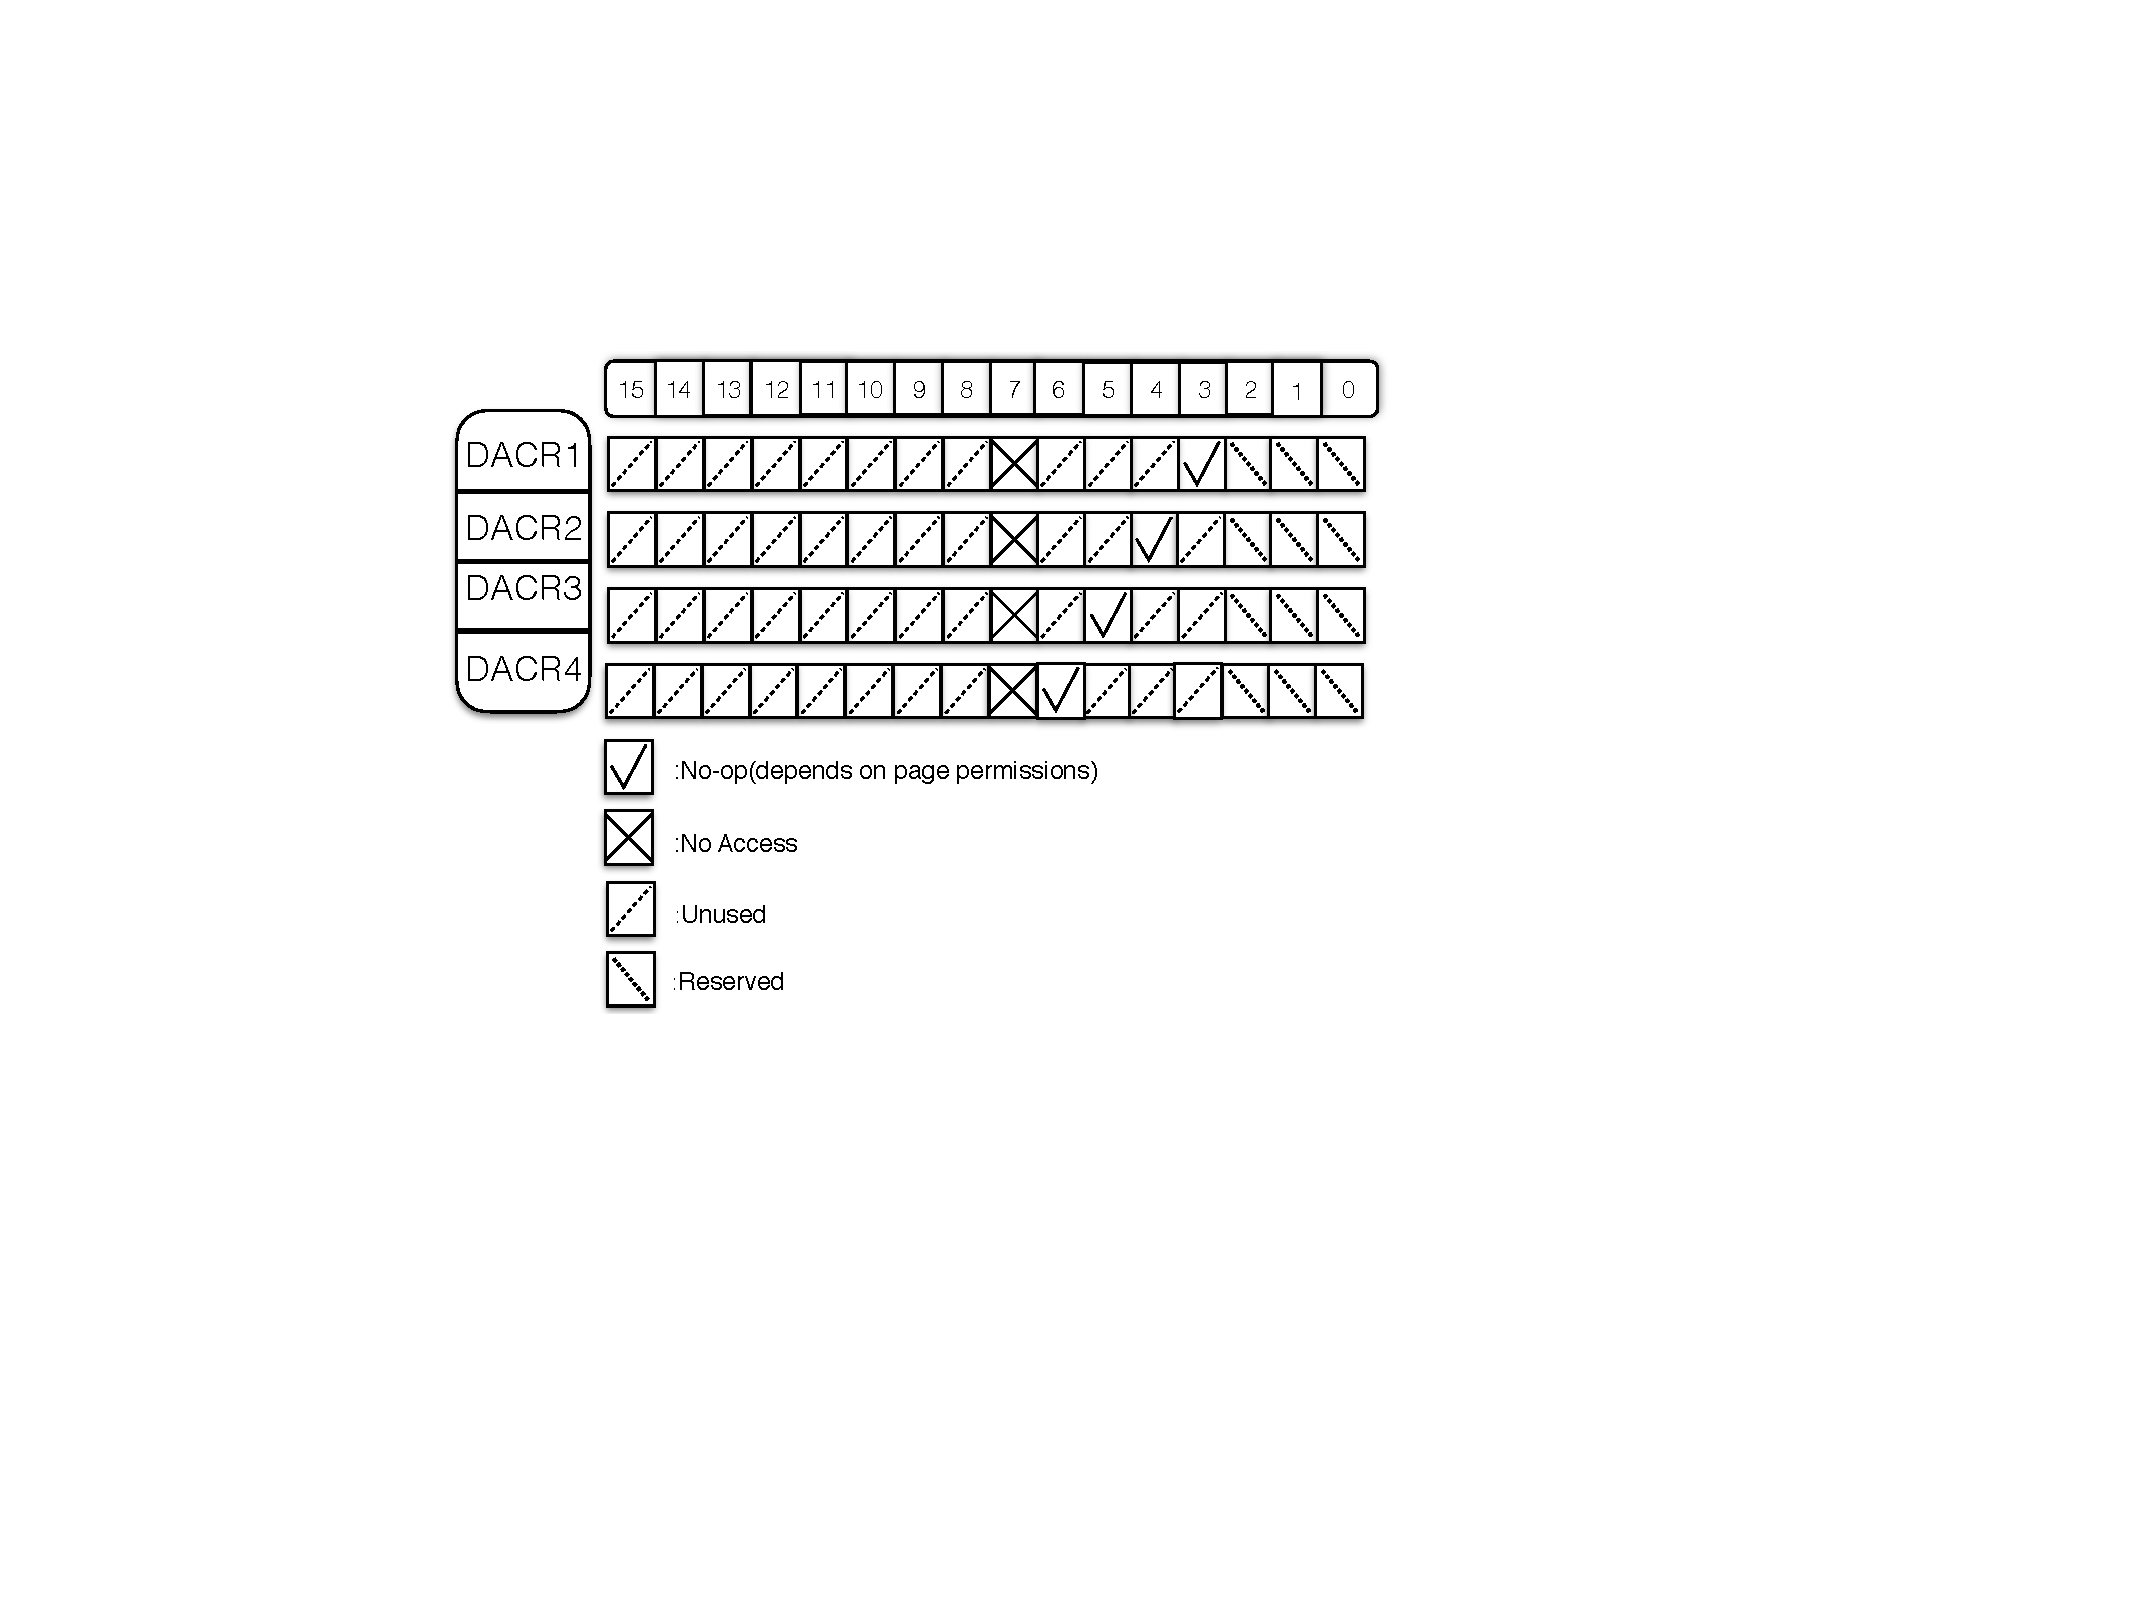
\includegraphics[width=\textwidth]{shreds/figures/dacr}
		\caption{The DACR setup for a quad-core system, where $k=4$. The first 3 domains ($Dom_{0}-Dom_{2}$) are reserved by Linux. Each core has a designated domain ($Dom_{3}-Dom_{6}$) that it may access when executing a shred. No CPU can access $Dom_{7}$. 
		 }
		\label{fig:dacr_setup}
	\end{minipage}
 \hfill
	\begin{minipage}[b]{0.4\textwidth}
		\centering	
		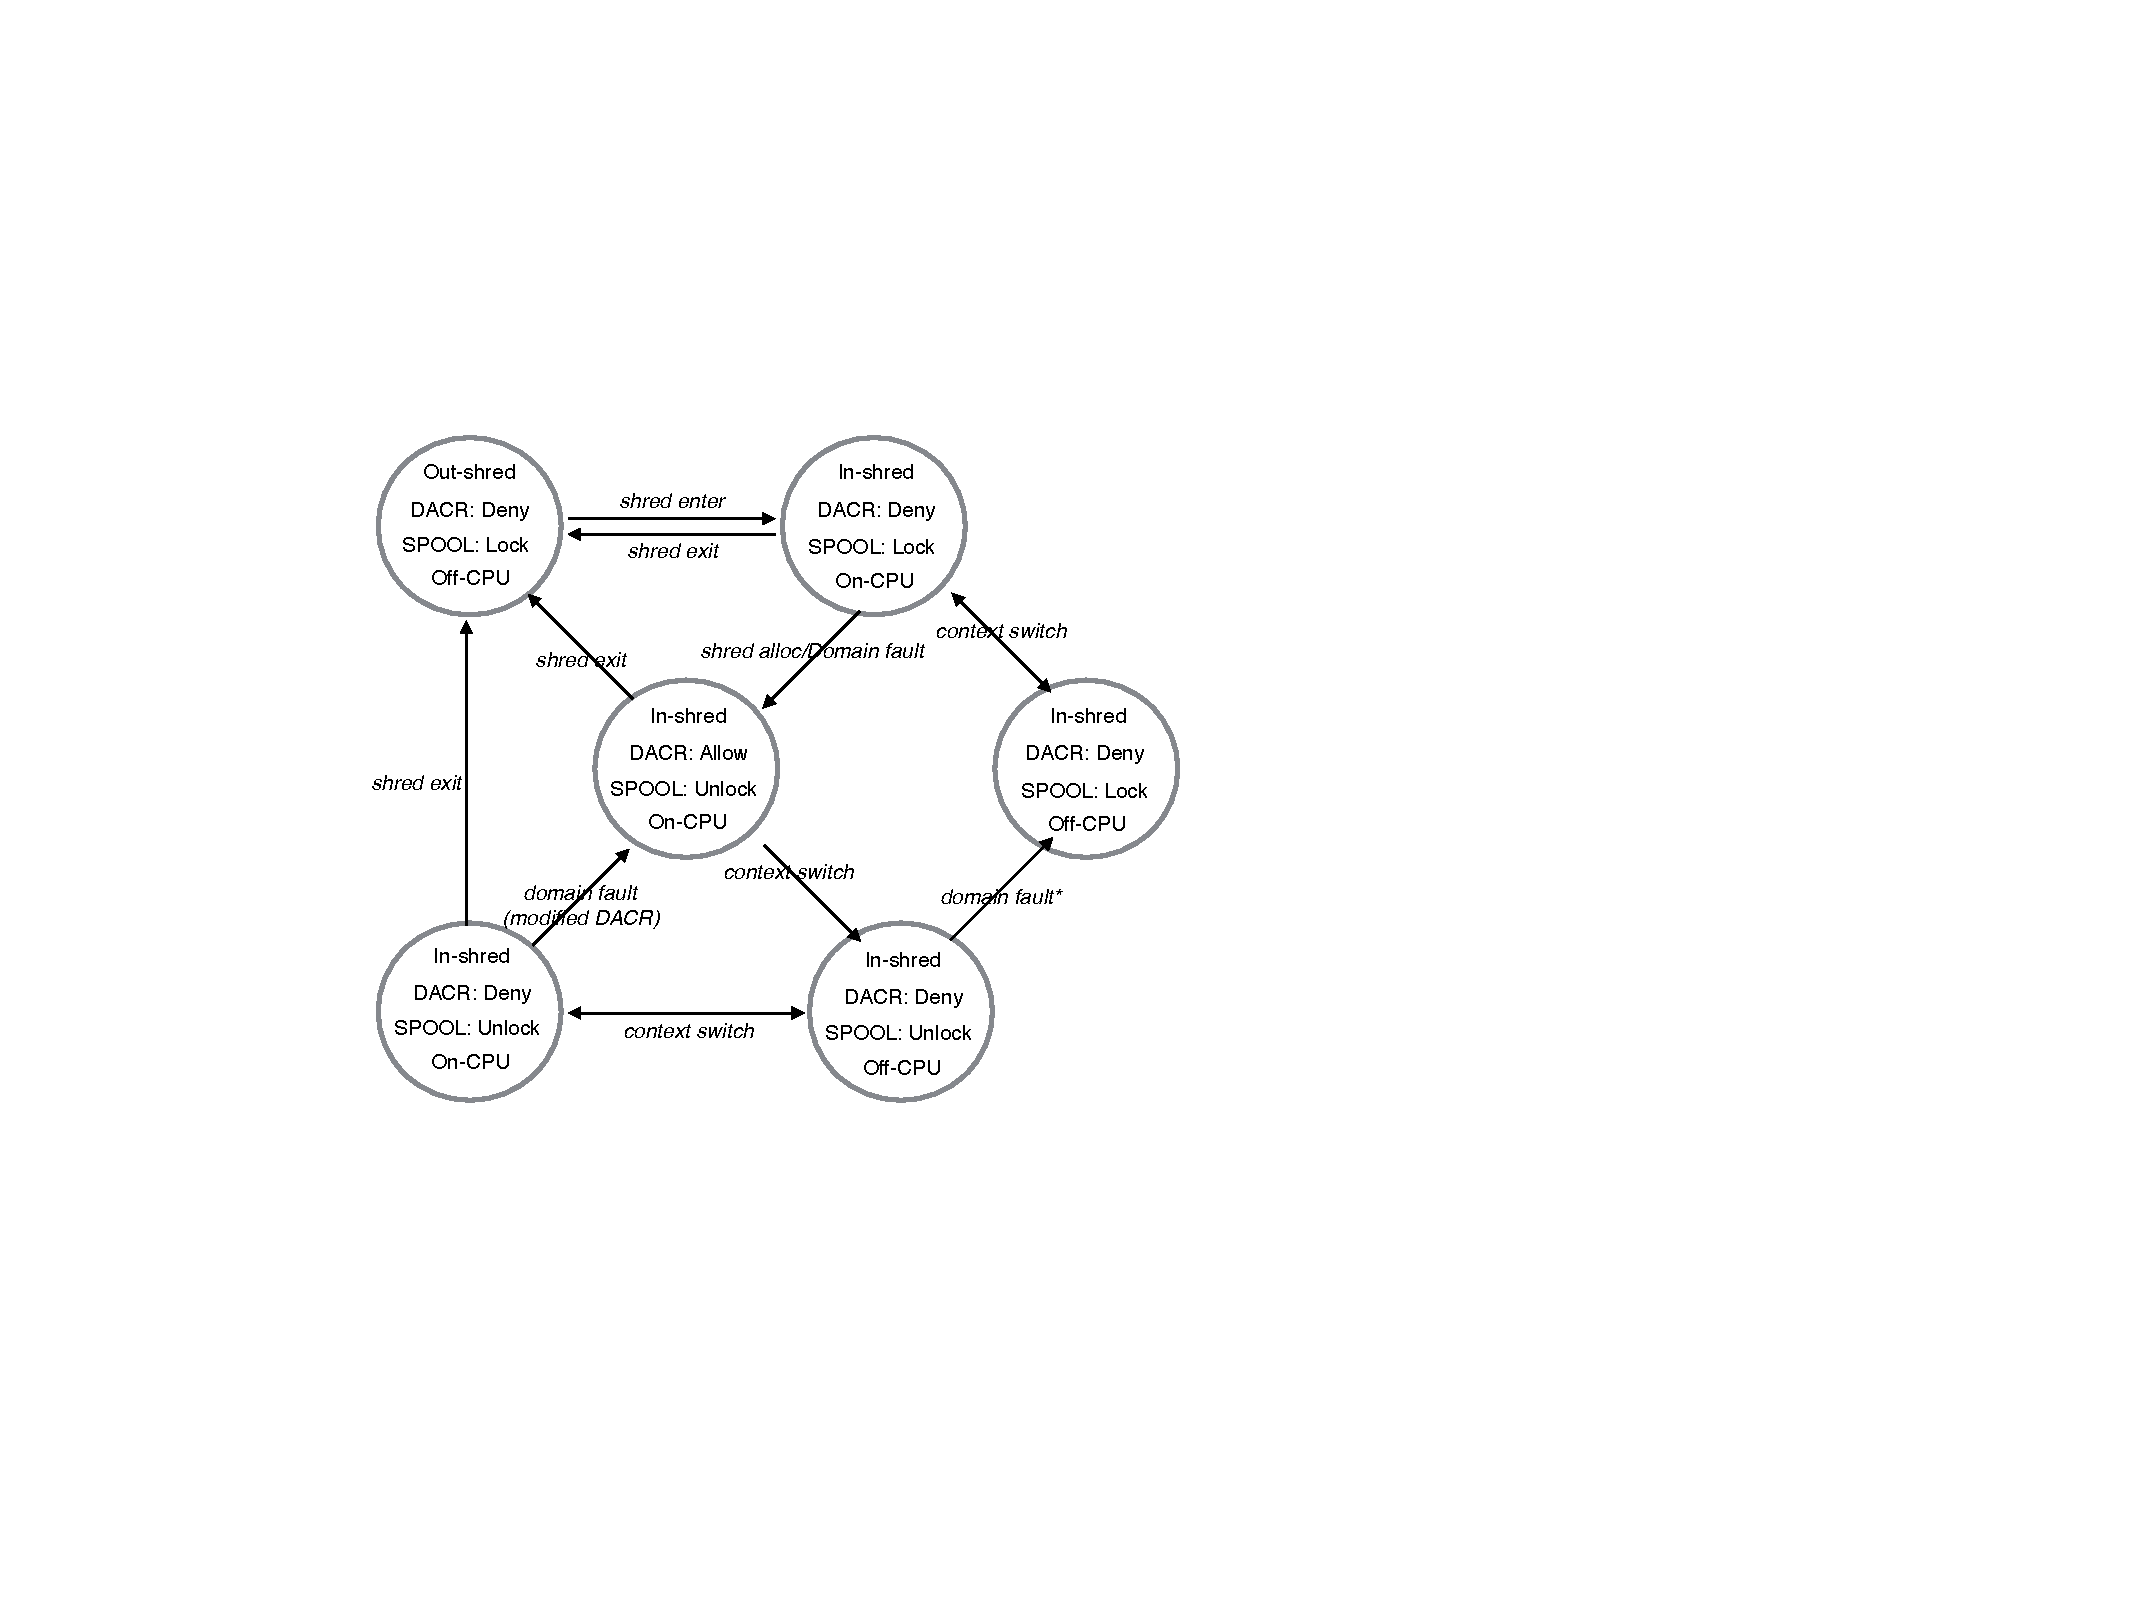
\includegraphics[width=\textwidth]{shreds/figures/shred_state_transition}
		\caption{A shred's transition of states}
		\label{fig:shredstat}
	\end{minipage}
\end{figure*}

S-driver uses the $k$ CPUs and the $k+1$ domains for executing shreds and protecting s-pools. 
When a shred starts or resumes its execution on $CPU_{i}$, S-driver assigns its associated s-pool to $Dom_{i}$, and therefore, the shred can freely access its s-pool while other concurrent threads, if any, cannot. 
When the shred terminates or is preempted, S-driver assigns its s-pool to $Dom_{k+1}$, which prevents any access to the pool from that moment on. 
As a result, S-driver allows or denies access to s-pools on a per-CPU basis, depending on if an associated shred occupies the CPU. 
Even if any malicious code manages to run concurrently alongside the shred inside the same process on another CPU, it cannot access the shred's s-pool without triggering domain faults. Thus, $P1$ is achieved. 

% performance and optimization 
It is reasonably efficient to switch s-pools to different domains upon shred entries and exits are. These operations do not involve heavy page table switches as process- or VM-based solutions do. They only require a shallow walk through of the first level page table and updates to the PDEs pointing to the s-pools in question. Besides, they do not trigger full TLB flushes as our design uses the per-address TLB eviction interface ({\tt flush\_tlb\_page}) and only invalidates the TLB entries related to the updated PDEs. 
To further reduce the overhead, we invent a technique called {\em lazy domain adjustment}: when a shred is leaving $CPU_{i}$, without adjusting any domain assignment, S-driver quickly changes the DACR to revoke the CPU's access to $Dom_{i}$ and lets the CPU's execution continue. It does not assign the s-pool used by the previous shred to $Dom_{k+1}$ until a domain fault happens (\ie another shred coming to the CPU and accessing its s-pool). The lazy domain adjustment avoids unnecessary domain changes and halves the already small overhead in some test cases.

%\begin{figure}[t]
%\begin{center}
%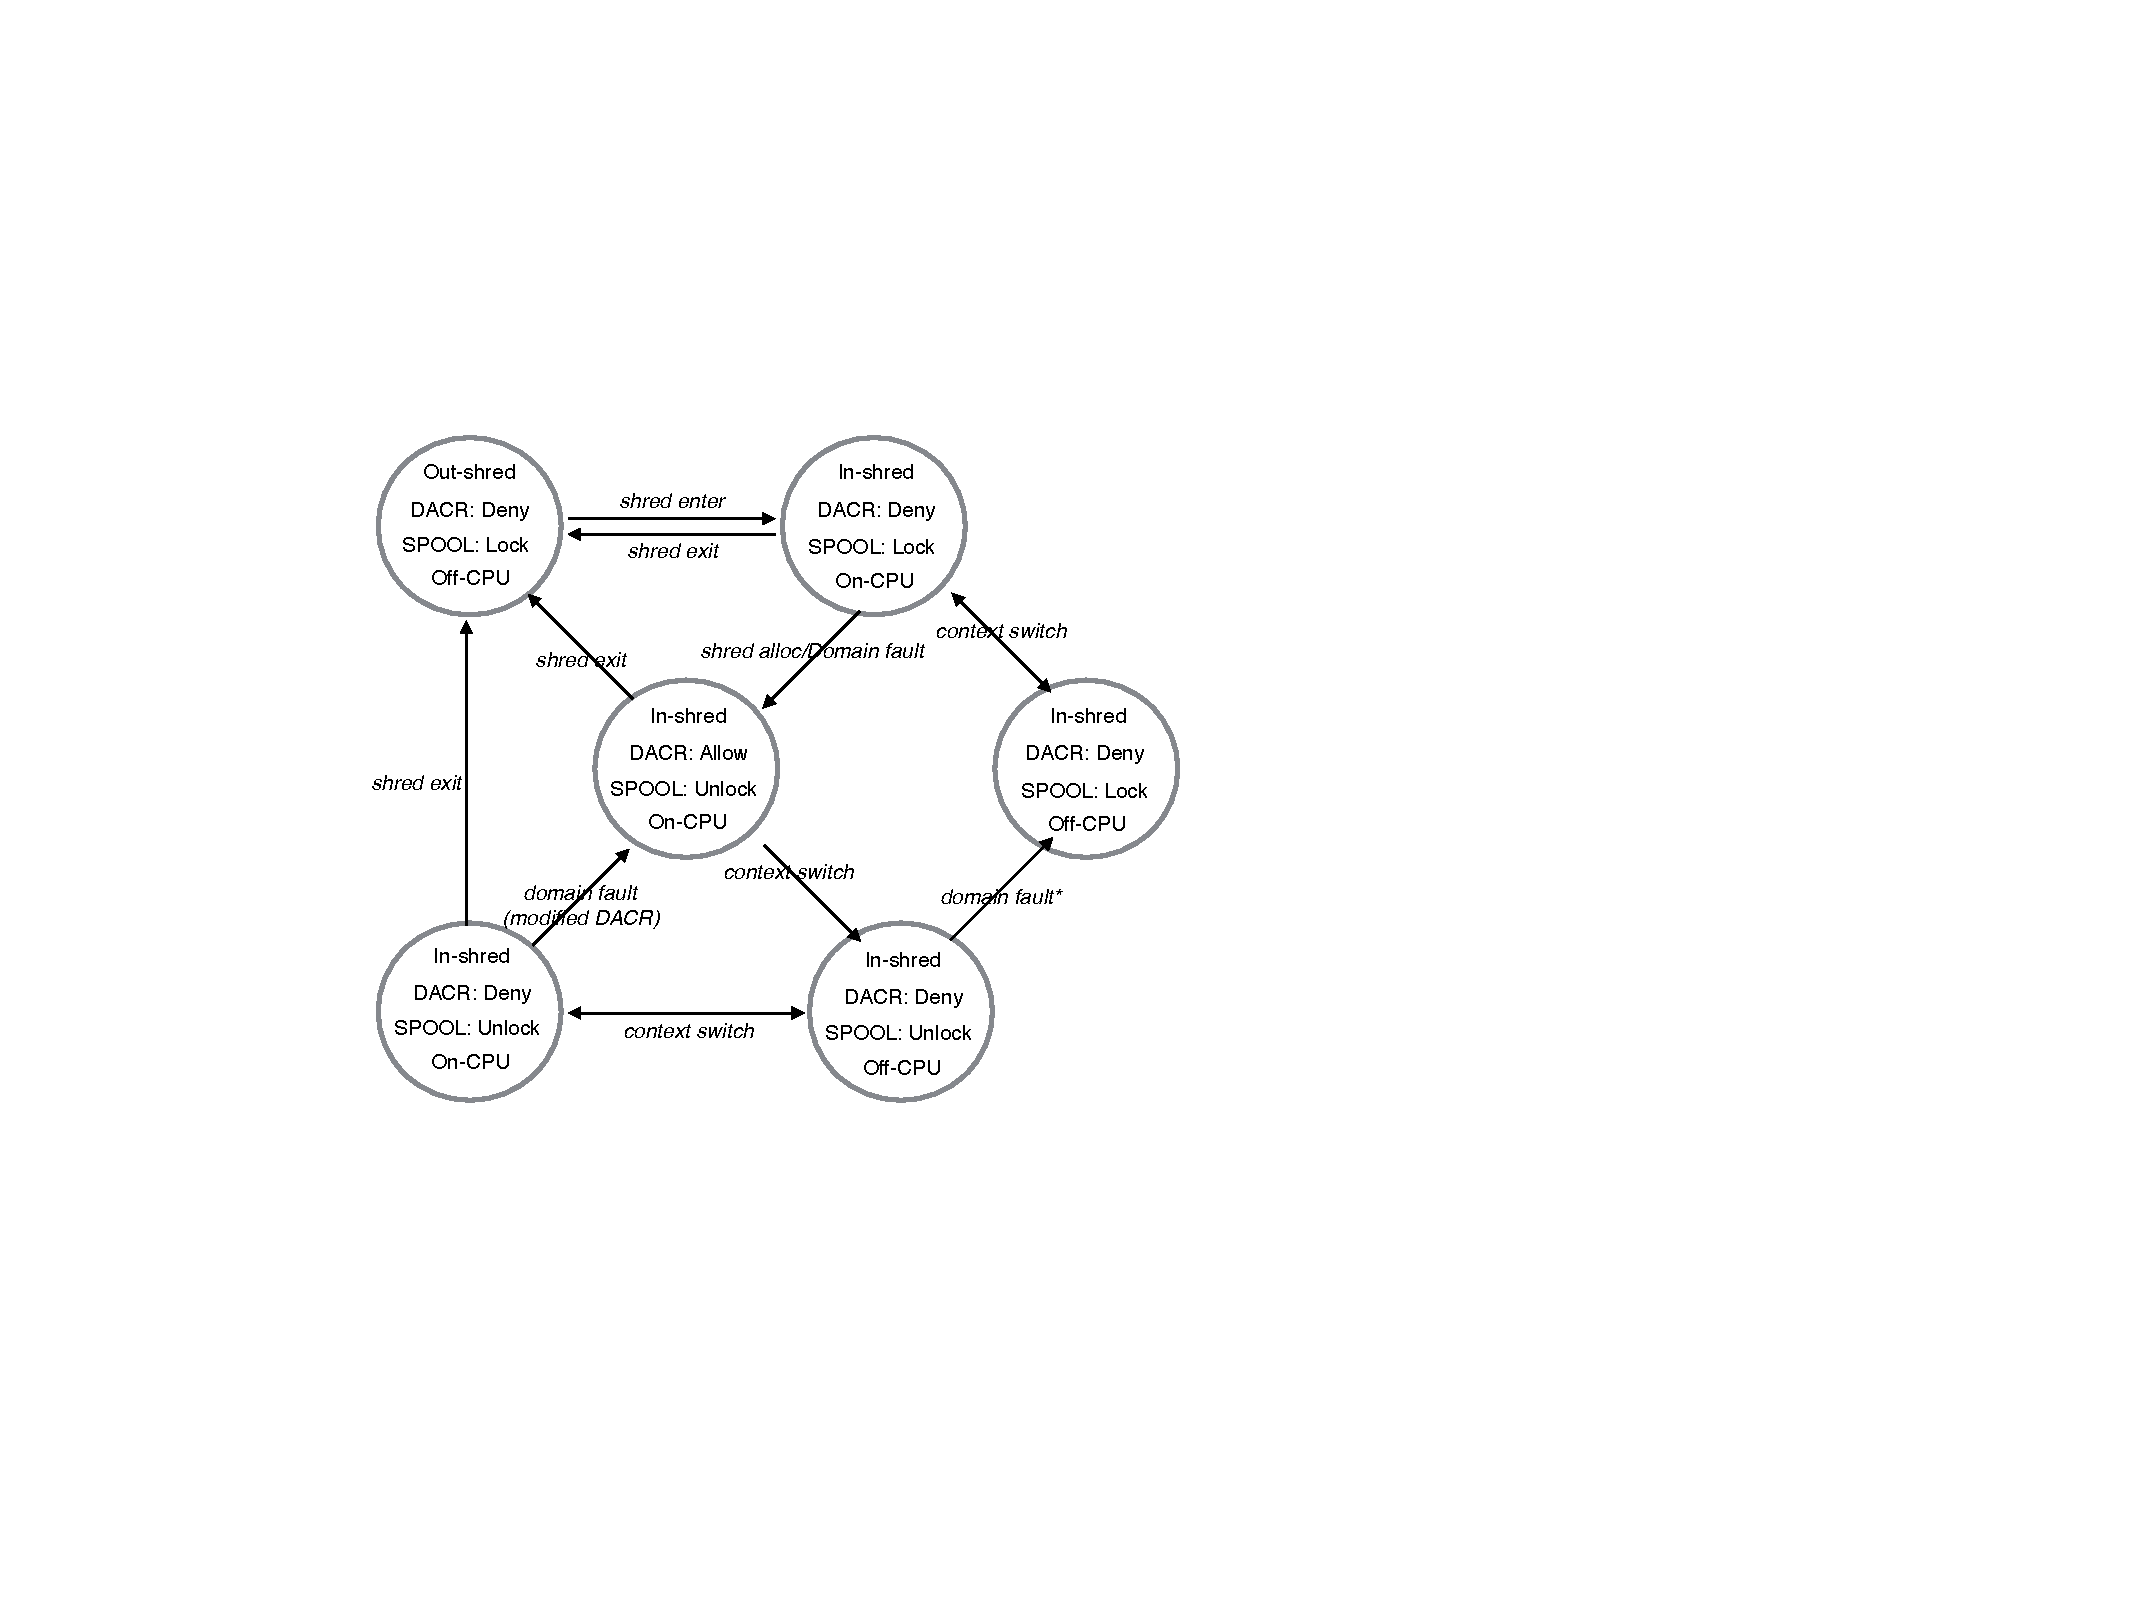
\includegraphics[scale=0.65]{shreds/figures/shred_state_transition}
%\caption{A shred's transition of states}
%\label{fig:shredstat}
%\end{center}
%\end{figure}

Figure~\ref{fig:shredstat} shows how S-driver orchestrates the transitions of a shred's states in response to the API calls, context switches, and domain faults. Each state is defined by a  combination of four properties:  

\begin{itemize}
\item $Shred$ = \{In-shred $|$ Out-shred\}: if the shred has started or exited. 
\item $DACR$ = \{Allow $|$ Deny\}: if the DACR allows or denies the current CPU to access its domain. 
\item $SPOOL$ = \{Lock $|$ Unlock\}: if the associated s-pool is locked or not. 
\item $CPU$ = \{On-CPU $|$ Off-CPU\}: if the shred is running on a CPU or not. 
\end{itemize}

The transition starts from the top, left circle, when the shred has not started and its s-pool is locked. After {\tt shred\_enter} is called, S-driver starts the shred, but it will not adjust the DACR or the s-pool access till a domain fault or a {\tt spool\_alloc} call due to the lazy domain adjustment in effect. When a context switch happens in the middle of the shred execution with unlocked DACR and s-pool, S-driver instantly sets the DACR to Deny but (safely) leaves the s-pool open. Later on, if a domain fault occurs, S-driver locks the previous s-pool because the fault means that the current code running on the CPU is in-shred and is trying to access its s-pool. If a domain fault never occurs till the shred regains the CPU, S-driver does not need to change any domain or s-pool settings, in which case the lazy domain adjustment saves two relatively heavy s-pool locking and unlocking operations. 
 
\point{Secure stacks for shreds}
%shadow stack support and switch 
Although S-compiler forbids unsanitized data flows from s-pools to unprotected memory regions, it has to allow in-shred code to copy s-pool data to local variables, which would be located in the regular stack and potentially accessible to in-process malicious code. 
To prevent secret leaks via stacks, S-driver creates a secure stack for each shred, allocated from its associated s-pool. When code execution enters a shred, S-driver transparently switches the stack without the application's knowledge: it copies the current stack frame to the secure stack and then overwrites the stack pointer. When the shred exits or encounters a signal to be handled outside of the shred, S-driver restores the regular stack.
As a result, local variables used by shreds never exist in regular stacks, and therefore cannot leak secrets.

\point{Runtime protection of shreds}
In addition to enabling and securing shreds and s-pools, S-driver also protects the inline reference monitor (IRM) that S-compiler plants in shred code. 
S-driver write-protects the memory pages containing the instrumented code and the associated data in memory.
It also pins the pages in s-pools in memory to prevent leaks via memory swap.  
Given that our threat model assumes the existence of in-process adversaries, S-driver also mediates the system calls that malicious code in user space may use to overwrite the page protection, dump physical memory via {\tt /dev/*mem}, disturb shreds via {\tt ptrace}, or load untrusted kernel modules. 
For each program using shreds, S-driver starts this mediation before loading the program code, avoiding pre-existing malicious code. 

S-driver's system call mediation also mitigates the attacks that steal secret data, not directly from s-pools, but from the I/O media where secret data are loaded or stored. 
For instance, instead of targeting the private key loaded in an s-pool, an in-process attacker may read the key file on disk. 
S-driver monitors file-open operations insides shreds. When the first time a file $F$ is accessed by a shred $S$, S-driver marks $F$ as a shred-private file and only allows shreds that share the same s-pool with $S$ to access $F$. This restriction is persistent and survives program and system reboots. 
As a result, an attacker can read $F$ only if she manages to intrude the program during its first run and access $F$ before a shred does. Although not completely preventing such attacks, S-driver makes them very difficult to succeed in reality. 
For a complete remedy, we envision a new primitive for in-shred code to encrypt and decrypt secret data with a persistent key assigned to each s-pool and automatically managed by S-driver. However, our current prototype does not support this primitive. 


It is worth noting that, although the system call mediation can prevent user-space malicious code that tries to break shreds via the system interfaces, it is a more intrusive and less configurable design choice than the well-known access control and capability frameworks, such as SELinux, AppArmor, and Capsicum~\cite{watson2010capsicum}. 
However, we leave the integration with those systems as future work because the system call mediation is easy to implement and is sufficient for the prototyping purpose. 

